\documentclass{beamer}
\usepackage[utf8]{inputenc}

\usetheme{Madrid}
\usecolortheme{default}
\usepackage{amsmath,amssymb,amsfonts,amsthm}
\usepackage{txfonts}
\usepackage{tkz-euclide}
\usepackage{listings}
\usepackage{adjustbox}
\usepackage{array}
\usepackage{tabularx}
\usepackage{gvv}
\usepackage{lmodern}
\usepackage{circuitikz}
\usepackage{tikz}
\usepackage{graphicx}
\usepackage{multicol}

\setbeamertemplate{page number in head/foot}[totalframenumber]

\usepackage{tcolorbox}
\tcbuselibrary{minted,breakable,xparse,skins}



\definecolor{bg}{gray}{0.95}
\DeclareTCBListing{mintedbox}{O{}m!O{}}{%
  breakable=true,
  listing engine=minted,
  listing only,
  minted language=#2,
  minted style=default,
  minted options={%
    linenos,
    gobble=0,
    breaklines=true,
    breakafter=,,
    fontsize=\small,
    numbersep=8pt,
    #1},
  boxsep=0pt,
  left skip=0pt,
  right skip=0pt,
  left=25pt,
  right=0pt,
  top=3pt,
  bottom=3pt,
  arc=5pt,
  leftrule=0pt,
  rightrule=0pt,
  bottomrule=2pt,
  toprule=2pt,
  colback=bg,
  colframe=orange!70,
  enhanced,
  overlay={%
    \begin{tcbclipinterior}
    \fill[orange!20!white] (frame.south west) rectangle ([xshift=20pt]frame.north west);
    \end{tcbclipinterior}},
  #3,
}
\lstset{
    language=C,
    basicstyle=\ttfamily\small,
    keywordstyle=\color{blue},
    stringstyle=\color{orange},
    commentstyle=\color{green!60!black},
    numbers=left,
    numberstyle=\tiny\color{gray},
    breaklines=true,
    showstringspaces=false,
}
%------------------------------------------------------------
%This block of code defines the information to appear in the
%Title page
\title %optional
{4.3.17}
\date{September 18,2025}


\author 
{Jnanesh Sathisha karmar - EE25BTECH11029}



\begin{document}



\frame{\titlepage}
\begin{frame}{Question}
 A plane passes through the points $\brak{2, 0, 0}, \brak{0, 3, 0} \text{and} \brak{0, 0, 4}$. The equation of the plane is \rule{2cm}{0.5pt}

\end{frame}



\begin{frame}{Equation}
 Given details
\begin{align}
    \vec{A}=\myvec{2\\0\\0}\  \vec{B}=\myvec{0\\3\\0}\ 
    \vec{C}=\myvec{0\\0\\4}
\end{align}
\end{frame}
\begin{frame}{Theoretical Solution}

The points for plane for 3 given points is:
\begin{align}
    \vec{n}^{\top}x=c
\end{align}
to find $\vec{n}$ by performing Gaussian elimination on the augmented  matrix:
\begin{align}
    \myvec{\vec{A}&\vec{B}&\vec{C}}^{\top}\vec{n}&=\myvec{1\\1\\1}\\
    \myvec{2&0&0\\0&3&0\\0&0&4}\vec{n}&=\myvec{1\\1\\1}\\
    \augvec{3}{1}{2&0&0&1\\0&3&0&1\\0&0&4&1}
    &\xrightarrow[\substack{R_2 \leftarrow R_2/3 \\ R_3 \leftarrow R_3/4}]{R_1 \leftarrow R_1/2}
    \augvec{3}{1}{1&0&0&\frac{1}{2}\\0&1&0&\frac{1}{3}\\0&0&1&\frac{1}{4}}
\end{align}
\end{frame}

\begin{frame}{Theoretical Solution}
This gives the solultion:
\begin{align}
    \vec{n}=\myvec{\frac{1}{2}\\ \frac{1}{3}\\ \frac{1}{4}}
\end{align}
Therefore the equation of plane is:
\begin{align}
    \myvec{\frac{1}{2}&\frac{1}{3}&\frac{1}{4}}^{\top}\vec{x}=1\\
    \myvec{6&4&3}^{\top}=12
\end{align}
\end{frame}






\begin{frame}[fragile]
    \frametitle{C Code (1) - Function to store the points }

    \begin{lstlisting}

#include <stdlib.h>


float* generate_plane_points(float x_min, float x_max, float y_min, float y_max, int num_steps) {
    if (num_steps <= 1) { 
        return NULL;
    }

    int total_points = num_steps * num_steps;
    float* points = (float*)malloc(total_points * 3 * sizeof(float));
    if (points == NULL) {
        return NULL; 
    }
    \end{lstlisting}
\end{frame}
\begin{frame}[fragile]
    \frametitle{C Code (1) - Function to store the points }

    \begin{lstlisting}
    float x_step_size = (x_max - x_min) / (num_steps - 1);
    float y_step_size = (y_max - y_min) / (num_steps - 1);

    int index = 0;
   
    for (int i = 0; i < num_steps; i++) {
        float x = x_min + i * x_step_size;
        
        for (int j = 0; j < num_steps; j++) {
            float y = y_min + j * y_step_size;

          
            float z = 4.0f - 2.0f * x - (4.0f / 3.0f) * y;

    \end{lstlisting}
\end{frame}
\begin{frame}[fragile]
    \frametitle{C Code (1) - Function to store the points }

    \begin{lstlisting}
            points[index++] = x;
            points[index++] = y;
            points[index++] = z;
        }
    }

    return points;
}


void free_points(float* points) {
    if (points != NULL) {
        free(points);
    }
}




    \end{lstlisting}
\end{frame}


\begin{frame}[fragile]
    \frametitle{Python Code - Using Shared Object}
    \begin{lstlisting}
import ctypes
import numpy as np
import matplotlib.pyplot as plt

lib = ctypes.CDLL("./plane.so")

lib.generate_plane_points.argtypes = [
    ctypes.c_float, ctypes.c_float,
    ctypes.c_float, ctypes.c_float,
    ctypes.c_int
]
lib.generate_plane_points.restype = ctypes.POINTER(ctypes.c_float)

lib.free_points.argtypes = [ctypes.POINTER(ctypes.c_float)]
lib.free_points.restype = None
NUM_STEPS = 50  
total_points = NUM_STEPS * NUM_STEPS
points_ptr = None


\end{lstlisting}
\end{frame}

\begin{frame}[fragile]
    \frametitle{Python Code - Using Shared Object}
    \begin{lstlisting}
try: 
    points_ptr = lib.generate_plane_points(-1.0, 3.0,-1.0, 4.0,NUM_STEPS)
    if not points_ptr:
        raise MemoryError("C function failed to allocate memory.")
   
    points_np = np.ctypeslib.as_array(points_ptr, shape=(total_points, 3))
    points_data = np.copy(points_np)
finally:
    if points_ptr:
        lib.free_points(points_ptr)
X = points_data[:, 0].reshape(NUM_STEPS, NUM_STEPS)
Y = points_data[:, 1].reshape(NUM_STEPS, NUM_STEPS)
Z = points_data[:, 2].reshape(NUM_STEPS, NUM_STEPS)


\end{lstlisting}
\end{frame}
\begin{frame}[fragile]
    \frametitle{Python Code - Using Shared Object}
    \begin{lstlisting}

fig = plt.figure(figsize=(10, 8))
ax = fig.add_subplot(projection='3d')


ax.plot_surface(X, Y, Z, cmap='plasma', alpha=0.8)
ax.scatter([2, 0, 0], [0, 3, 0], [0, 0, 4], color='black', s=100, label='Defining Points')
ax.text(2.1,0.1,0.1,"A",color="black")
ax.text(0.1,3.1,0.1,"B",color="black")
ax.text(0.1,0.1,4.1,"C",color="black")
ax.set_xlabel('X-axis')
ax.set_ylabel('Y-axis')
ax.set_zlabel('Z-axis')
ax.set_title('Simplified Plane Generation')
ax.legend()
plt.savefig("./figs/plane.png")
subprocess.run(shlex.split('termux-open ../figs/parallelogram.png'))
plt.show()

\end{lstlisting}
\end{frame}



\begin{frame}{Plot-Using Both C and Python}
    \centering
    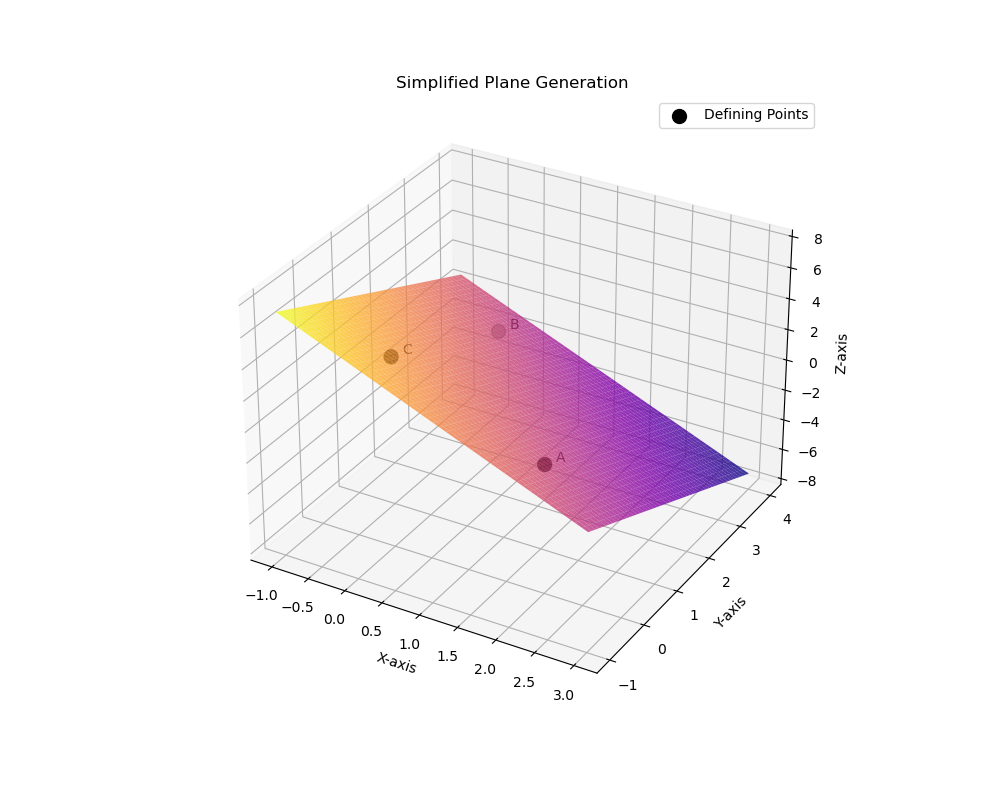
\includegraphics[width=\columnwidth, height=0.8\textheight, keepaspectratio]{figs/plane.png}     
\end{frame}

\begin{frame}[fragile]
    \frametitle{Python Code}
    \begin{lstlisting}
import numpy as np
import matplotlib.pyplot as plt

def plot_plane_from_points():
    p1 = np.array([2, 0, 0])
    p2 = np.array([0, 3, 0])
    p3 = np.array([0, 0, 4])

    x_range = np.linspace(-1, 4, 20)
    y_range = np.linspace(-1, 4, 20)
    X, Y = np.meshgrid(x_range, y_range)

    Z = 4 - 2 * X - (4 / 3) * Y

    fig = plt.figure(figsize=(10, 8))
    ax = fig.add_subplot(projection='3d')

\end{lstlisting}
\end{frame}
\begin{frame}[fragile]
    \frametitle{Python Code}
    \begin{lstlisting}
    ax.plot_surface(X, Y, Z, alpha=0.7, cmap='plasma', edgecolor='none')

    ax.scatter(p1[0], p1[1], p1[2], color='red', s=120, label='(2,0,0)', depthshade=False)
    ax.scatter(p2[0], p2[1], p2[2], color='red', s=120, label='(0,3,0)', depthshade=False)
    ax.scatter(p3[0], p3[1], p3[2], color='red', s=120, label='(0,0,4)', depthshade=False)
    ax.text(2.1,0.1,0.1,"A",color="black")
    ax.text(0.1,3.1,0.1,"B",color="black")
    ax.text(0.1,0.1,4.1,"C",color="black")



\end{lstlisting}
\end{frame}
\begin{frame}[fragile]
    \frametitle{Python Code}
    \begin{lstlisting}
    ax.set_xlabel('X-axis')
    ax.set_ylabel('Y-axis')
    ax.set_zlabel('Z-axis')
    ax.set_title('Plane Passing Through Three Points')
    ax.legend()
    ax.set_xlim([-1, 4])
    ax.set_ylim([-1, 4])
    ax.set_zlim([-1, 6])
    plt.savefig("./figs/plane2.png")
    plt.show()
    subprocess.run(shlex.split('termux-open ../figs/parallelogram.png'))

if __name__ == '__main__':
    plot_plane_from_points()
\end{lstlisting}
\end{frame}



\begin{frame}{Plot-Using only Python}
    \centering
    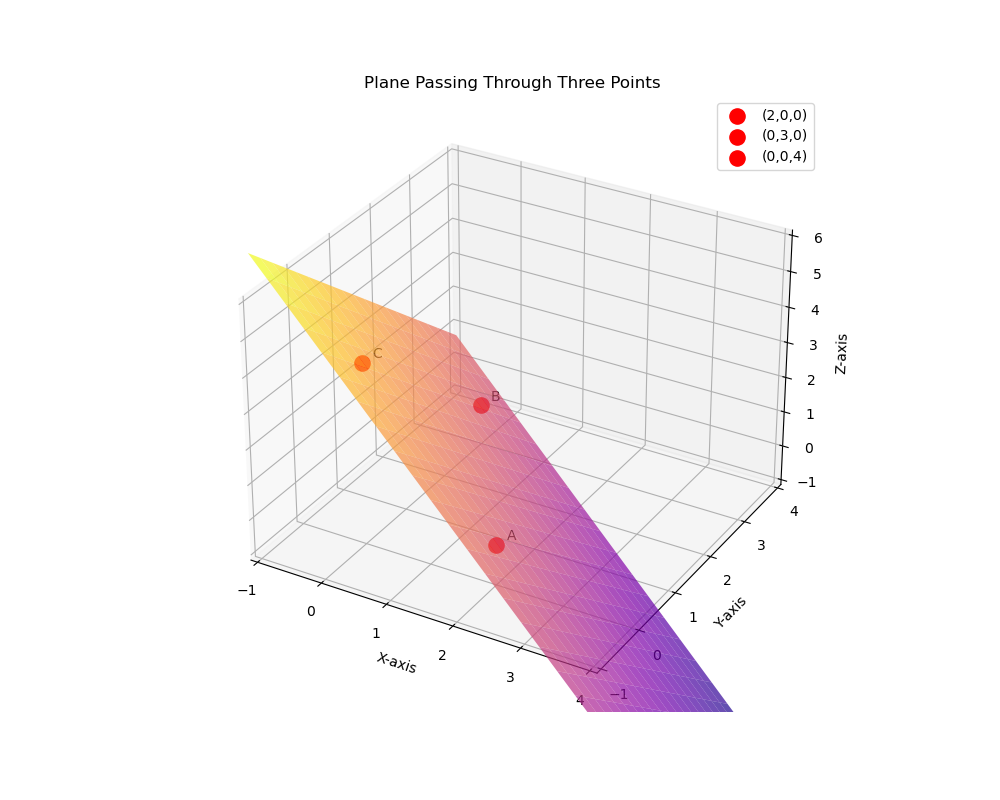
\includegraphics[width=\columnwidth, height=0.8\textheight, keepaspectratio]{figs/plane2.png}     
\end{frame}


\end{document}